\subsection{Arquitectura del Sistema}

La arquitectura implementada en el Trabajo Terminal 1 se enfoca en establecer una base sólida y escalable para la aplicación web. Esta sección documenta el estado actual de la implementación, dejando clara la separación de responsabilidades entre módulos y la organización de rutas por tipo de usuario.

\subsubsection{Visión General de la Arquitectura}

La aplicación backend implementa una arquitectura en capas que separa claramente las responsabilidades de acceso a datos, lógica de negocio y gestión de rutas. El sistema está desarrollado con FastAPI como framework principal, proporcionando una base robusta para la gestión de solicitudes HTTP y la validación automática de datos.

La arquitectura se organiza en los siguientes componentes principales:

\begin{itemize}
    \item \textbf{Capa de Acceso a Datos (DAO):} Encargada de todas las operaciones con la base de datos SQL Server
    \item \textbf{Capa de Autenticación y Autorización:} Gestión de tokens JWT y control de acceso basado en roles
    \item \textbf{Capa de Rutas (Routers):} Endpoints organizados por tipo de actor (Alumno, Tutor, Autenticación)
    \item \textbf{Capa de Validación (Schemas):} Modelos Pydantic que aseguran la integridad de datos entrantes
\end{itemize}

Esta separación en capas facilita el mantenimiento, las pruebas unitarias y futuras mejoras del sistema, especialmente la integración de los módulos OCR y NLP en TT2.

\subsubsection{Patrón de Diseño DAO (Data Access Object)}

El patrón DAO implementado en este proyecto abstrae completamente la lógica de acceso a datos, permitiendo una separación clara entre la lógica de negocio y la persistencia de datos en SQL Server. Esta arquitectura facilita el mantenimiento, las pruebas y futuras migraciones de bases de datos.

\subsubsection{Estructura del DAO}

El proyecto organiza las funciones DAO en módulos específicos para cada dominio del sistema:

\begin{itemize}
    \item \texttt{dao\_alumno.py}: Operaciones relacionadas con perfiles y datos de alumnos
    \item \texttt{dao\_tutor.py}: Operaciones de gestión de alumnos y reportes de tutores
    \item \texttt{dao\_auth.py}: Operaciones de autenticación y contraseñas
\end{itemize}

Cada módulo DAO encapsula las consultas SQL y la conexión a la base de datos, exponiendo funciones con nombres descriptivos que reflejan la operación que realizan.

\begin{lstlisting}[language=Python, label=lst:dao_estructura, caption={Estructura de funciones DAO por módulo}]
# dao_alumno.py
def actualizar_info_alumno_dao(nombre, apellido_paterno, 
                                apellido_materno, grupo, id_usuario)
def actualizar_password_alumno_dao(nueva_contrasena, id_usuario)
def verificar_estado_tutor_dao(id_usuario)
def registrar_intento_dao(ejercicio_tutor_id, imagen_codificada, 
                          id_usuario)
def obtener_ejercicios_proximos_dao(id_usuario)
def obtener_ejercicios_completados_dao(id_usuario)
def obtener_ejercicios_vencidos_dao(id_usuario)

# dao_tutor.py
def registrar_alumno_dao(alumno_data, hashed_password)
def obtener_alumnos_por_tutor_dao(id_tutor)
def obtener_alumnos_en_riesgo_dao(id_tutor)
def calificar_intento_dao(id_intento, calificacion, 
                          retroalimentacion)
def activar_ejercicio_tutor_dao(id_ejercicio, id_usuario, fecha_fin)
def get_ejercicios_dao()

# dao_auth.py
def login_dao(username)
def register_dao(username, email, hashed_password, nombre, apellido)
def obtener_hash_contrasena_dao(id_usuario)
\end{lstlisting}

\textbf{Ventajas de esta aproximación:}

\begin{itemize}
    \item Centraliza todas las operaciones de base de datos en un único lugar
    \item Facilita cambios en la implementación de consultas SQL sin afectar las rutas
    \item Permite reutilizar código de acceso a datos en múltiples endpoints
    \item Mejora significativamente la testabilidad del código
    \item Reduce el riesgo de inyección SQL mediante el uso consistente de parámetros preparados
\end{itemize}

\subsubsection{Ejemplo de Implementación DAO}

A continuación se muestra un ejemplo de cómo los DAOs abstraen la lógica de base de datos:

\begin{lstlisting}[language=Python, label=lst:dao_ejemplo, caption={Ejemplo de función DAO para obtener ejercicios próximos}]
def obtener_ejercicios_proximos_dao(id_usuario):
    conn = connect_to_database()
    if not conn:
        raise ConnectionError("Error de conexion a la BD")
    cursor = conn.cursor()
    try:
        query = """
            -- Consulta SQL para obtener ejercicios proximos asignados a un alumno
        """
        # Resto de la implementacion con manejo de errores y retorno de resultados
    finally:
        cursor.close()
        conn.close()
\end{lstlisting}

\subsubsection{Organización de Rutas por Actor}

El backend organiza los endpoints en tres grupos principales basados en el tipo de usuario y el nivel de autorización requerido. La estructura base de rutas es \texttt{/api/\{actor\}/\{endpoint\}}, donde \textit{actor} puede ser \texttt{alumno}, \texttt{tutor} o \texttt{auth}.

\subsubsection{Rutas de Autenticación (Prefix: /api/auth)}

El módulo de autenticación (implementado en \texttt{Control/auth.py}) gestiona la creación de sesiones, login y validación de credenciales. Los endpoints en esta sección no requieren autenticación previa.

\begin{table}[H]
\centering
\caption{Endpoints de Autenticación}
\begin{tabular}{|l|c|l|}
\hline
\textbf{Método} & \textbf{Endpoint} & \textbf{Descripción} \\
\hline
POST & \texttt{/api/auth/login} & Autenticar usuario y obtener token JWT \\
\hline
POST & \texttt{/api/auth/register} & Registrar nueva cuenta de tutor \\
\hline
POST & \texttt{/api/auth/refresh} & Renovar token JWT expirado \\
\hline
\end{tabular}
\end{table}

El login verifica las credenciales contra la tabla \texttt{Usuario} y retorna un token JWT que incluye el \texttt{id\_usuario}, \texttt{tipo\_usuario}, \texttt{id\_estatus} e identificadores específicos del rol (\texttt{id\_tutor} o \texttt{id\_alumno}).

\subsubsection{Rutas para Alumnos (Prefix: /api/alumno)}

Estos endpoints (implementados en \texttt{Control/alumno.py}) permiten a los alumnos interactuar con la plataforma de práctica. Todos requieren autenticación y verifican que el usuario sea de tipo \texttt{alumno} mediante el decorador \texttt{@require\_alumno}.

\begin{table}[H]
\centering
\caption{Endpoints para Alumnos}
\begin{tabular}{|l|c|l|}
\hline
\textbf{Método} & \textbf{Endpoint} & \textbf{Descripción} \\
\hline
PUT & \texttt{/api/alumno/info} & Actualizar información del perfil \\
\hline
PUT & \texttt{/api/alumno/act/password} & Cambiar contraseña \\
\hline
GET & \texttt{/api/alumno/estado-tutor} & Verificar si tutor está activo \\
\hline
POST & \texttt{/api/alumno/intento} & Registrar nuevo intento de práctica \\
\hline
GET & \texttt{/api/alumno/ejercicios/proximos} & Listar ejercicios pendientes \\
\hline
GET & \texttt{/api/alumno/ejercicios/completados} & Obtener historial de intentos \\
\hline
GET & \texttt{/api/alumno/ejercicios/vencidos} & Listar ejercicios vencidos \\
\hline
\end{tabular}
\end{table}

\subsubsection{Rutas para Tutores (Prefix: /api/tutor)}

Estos endpoints (implementados en \texttt{Control/tutor.py}) permiten a los tutores gestionar sus grupos de alumnos, revisar su progreso y activar ejercicios. Todos requieren autenticación y verifican que el usuario sea de tipo \texttt{tutor} mediante el decorador \texttt{@require\_tutor}.

\begin{table}[H]
\centering
\caption{Endpoints para Tutores - Gestión de Alumnos}
\begin{tabular}{|l|c|l|}
\hline
\textbf{Método} & \textbf{Endpoint} & \textbf{Descripción} \\
\hline
POST & \texttt{/api/tutor/registrar} & Crear nuevo alumno \\
\hline
GET & \texttt{/api/tutor/alumnos/\{id\_tutor\}} & Listar alumnos asignados \\
\hline
PUT & \texttt{/api/tutor/baja/\{id\_alumno\}} & Dar de baja a alumno \\
\hline
GET & \texttt{/api/tutor/riesgo/\{id\_tutor\}} & Alumnos con bajo desempeño \\
\hline
GET & \texttt{/api/tutor/regular/\{id\_tutor\}} & Alumnos con desempeño regular \\
\hline
GET & \texttt{/api/tutor/excelencia/\{id\_tutor\}} & Alumnos con desempeño alto \\
\hline
GET & \texttt{/api/tutor/progreso/\{id\_tutor\}} & Gráfico de progreso general \\
\hline
\end{tabular}
\end{table}

\begin{table}[H]
\centering
\caption{Endpoints para Tutores - Gestión de Perfil}
\begin{tabular}{|l|c|l|}
\hline
\textbf{Método} & \textbf{Endpoint} & \textbf{Descripción} \\
\hline
PUT & \texttt{/api/tutor/act/nombre} & Actualizar nombre \\
\hline
PUT & \texttt{/api/tutor/act/correo} & Cambiar correo electrónico \\
\hline
PUT & \texttt{/api/tutor/act/password} & Cambiar contraseña \\
\hline
DELETE & \texttt{/api/tutor/eliminar} & Desactivar cuenta \\
\hline
\end{tabular}
\end{table}

\begin{table}[H]
\centering
\caption{Endpoints para Tutores - Gestión de Intentos y Ejercicios}
\begin{tabular}{|l|c|l|}
\hline
\textbf{Método} & \textbf{Endpoint} & \textbf{Descripción} \\
\hline
GET & \texttt{/api/tutor/intentos/\{id\_tutor\}} & Obtener intentos de todos sus alumnos \\
\hline
PUT & \texttt{/api/tutor/calificar/\{id\_intento\}} & Asignar calificación y retroalimentación \\
\hline
GET & \texttt{/api/tutor/ejercicios} & Listar todos los ejercicios disponibles \\
\hline
GET & \texttt{/api/tutor/ejercicios/\{id\_usuario\}} & Ejercicios activados por el tutor \\
\hline
POST & \texttt{/api/tutor/ejercicio/activar} & Activar ejercicio para sus alumnos \\
\hline
DELETE & \texttt{/api/tutor/ejercicio/desactivar/\{id\}/\{id\_ej\}} & Desactivar ejercicio \\
\hline
\end{tabular}
\end{table}

\subsection{Diseño de Tokens JWT y Control de Acceso}

Los tokens JWT se utilizan para autenticar y autorizar las solicitudes posteriores al login. Cada token contiene información sobre el usuario y su rol, permitiendo al servidor validar permisos sin consultar la base de datos en cada solicitud.

\subsubsection{Estructura del Token JWT}

\begin{lstlisting}[language=JSON, label=lst:jwt_payload, caption={Estructura del payload de un token JWT generado por el sistema}]
{
  "sub": "id_usuario",
  "username": "usuario_tutor",
  "tipo_usuario": "tutor",
  "id_estatus": 1,
  "id_tutor": 5,
  "id_alumno": null,
  "iat": 1705267200,
  "exp": 1705270800
}
\end{lstlisting}

El campo \texttt{sub} (subject) contiene el \texttt{id\_usuario}, que es el identificador único en el sistema. Los campos \texttt{id\_tutor} e \texttt{id\_alumno} se incluyen solo si aplican al tipo de usuario, facilitando las validaciones posteriores.

\subsubsection{Control de Acceso Basado en Roles (RBAC)}

El sistema implementa un control de acceso basado en roles que asegura que cada usuario solo pueda acceder a los endpoints correspondientes a su rol. Las validaciones se realizan mediante decoradores llamados en cada endpoint.

\begin{itemize}
    \item \textbf{Rol Alumno (\texttt{tipo\_usuario='alumno'}):} 
    \begin{itemize}
        \item Acceso solo a \texttt{/api/alumno/\{endpoint\}}
        \item Puede ver y registrar intentos de ejercicios asignados
        \item Puede actualizar su perfil
    \end{itemize}
    \item \textbf{Rol Tutor (\texttt{tipo\_usuario='tutor'}):} 
    \begin{itemize}
        \item Acceso a \texttt{/api/tutor/\{endpoint\}}
        \item Puede registrar, ver y gestionar sus alumnos
        \item Puede calificar intentos de sus alumnos
        \item Puede activar y desactivar ejercicios
    \end{itemize}
\end{itemize}

La validación del rol se realiza mediante decoradores en FastAPI que verifican el token JWT:

\begin{lstlisting}[language=Python, label=lst:rbac_decorator, caption={Validación de rol mediante decoradores - Alumno}]
from fastapi import Depends
from Control.dependencies import require_alumno

@router.put("/info")
def actualizar_info_alumno(
    data: AlumnoUpdate, 
    current_user: dict = Depends(require_alumno)
):
    # current_user contiene la informacion decodificada del JWT
    id_usuario = current_user["id_usuario"]
    # Logica del endpoint usando el DAO
    actualizar_info_alumno_dao(data.nombre, data.apellido_paterno,
                               data.apellido_materno, data.grupo, 
                               id_usuario)
    return {"message": "Informacion actualizada correctamente"}
\end{lstlisting}

\begin{lstlisting}[language=Python, label=lst:rbac_decorator_tutor, caption={Validación de rol mediante decoradores - Tutor}]
from fastapi import Depends
from Control.dependencies import require_tutor

@router.get("/alumnos/{id_tutor}")
def obtener_alumnos_por_tutor(
    id_tutor: int, 
    current_user: dict = Depends(require_tutor)
):
    # Validacion adicional: verificar que el tutor solo vea sus propios alumnos
    if current_user["id_usuario"] != id_tutor:
        raise HTTPException(status_code=403, 
                          detail="No tiene permiso para ver alumnos de otro tutor")
    
    return obtener_alumnos_por_tutor_dao(id_tutor)
\end{lstlisting}

La función \texttt{require\_alumno} y \texttt{require\_tutor} en el módulo \texttt{Control/dependencies.py} decodifica el token JWT y verifica que sea válido y del tipo correcto.

\subsubsection{Flujo Completo de Autenticación}

El flujo de autenticación y autorización sigue estos pasos:

\begin{enumerate}
    \item El usuario proporciona credenciales (\texttt{username} y \texttt{password}) al endpoint \texttt{POST /api/auth/login}
    \item El servidor:
    \begin{enumerate}
        \item Valida que el usuario existe usando \texttt{login\_dao(username)}
        \item Verifica que la contraseña es correcta comparándola contra el hash almacenado
        \item Obtiene el \texttt{tipo\_usuario} (\texttt{alumno} o \texttt{tutor})
        \item Genera un token JWT que incluye \texttt{id\_usuario}, \texttt{tipo\_usuario}, \texttt{id\_estatus}, e identificadores adicionales
        \item Retorna el token en una respuesta \texttt{LoginResponse}
    \end{enumerate}
    \item El cliente almacena el token en su almacenamiento local
    \item En posteriores solicitudes, el cliente envía el token en el header: \texttt{Authorization: Bearer <token>}
    \item El servidor valida el token usando el decorador \texttt{Depends(require\_alumno)} o \texttt{Depends(require\_tutor)}
    \item Si el token es válido y el usuario tiene permiso, la solicitud se procesa
    \item Si hay un error de autenticación o autorización, se retorna un \texttt{HTTPException} con código 401 o 403
\end{enumerate}

\subsection{Contratos de Datos (Schemas Pydantic)}

Los contratos de datos definen la estructura de los objetos que se intercambian entre el cliente y el servidor, así como entre diferentes módulos del sistema. Esto asegura que todos los componentes trabajen con la misma representación de datos y permite la validación automática.

\subsubsection{Esquemas de Autenticación}

\begin{lstlisting}[language=Python, label=lst:schemas_auth, caption={Schemas de autenticación}]
class LoginRequest(BaseModel):
    username: str
    password: str

class LoginResponse(BaseModel):
    message: str
    token: str

class RegisterRequest(BaseModel):
    nombre: str
    apellido: str
    username: str  # Validacion: min 6 caracteres, alfanumericos
    email: str
    password: str  # Validacion: min 8 caracteres, complejidad

class PasswordUpdate(BaseModel):
    contrasena_actual: str
    nueva_contrasena: str

class DeleteAccount(BaseModel):
    contrasena_actual: str
\end{lstlisting}

\subsubsection{Esquemas de Alumno}

\begin{lstlisting}[language=Python, label=lst:schemas_alumno, caption={Schemas de datos de Alumno}]
class AlumnoCreate(BaseModel):
    nombre: str
    apellido_paterno: str
    apellido_materno: Optional[str] = None
    usuario: str
    contrasena: str
    grado: str
    grupo: Optional[str] = None
    id_tutor: int

class AlumnoUpdate(BaseModel):
    nombre: str
    apellido_paterno: str
    apellido_materno: Optional[str]
    grupo: Optional[str]

class AlumnoResponse(BaseModel):
    id_alumno: int
    nombre: str
    apellido_paterno: str
    apellido_materno: Optional[str]
    usuario: str
    grado: str
    grupo: Optional[str]

class AlumnoProgresoResponse(BaseModel):
    id_alumno: int
    nombre: str
    apellido_paterno: str
    apellido_materno: str
    promedio_ortografia: Decimal
    promedio_legibilidad: Decimal

class IntentoCreate(BaseModel):
    id_ejercicio_tutor: int
    imagen_codificada: str
\end{lstlisting}

\subsubsection{Esquemas de Tutor}

\begin{lstlisting}[language=Python, label=lst:schemas_tutor, caption={Schemas de datos de Tutor}]
class TutorUpdate(BaseModel):
    nombre: str

class EmailUpdate(BaseModel):
    correo: str
    contrasena_actual: str

class CalificarIntentoRequest(BaseModel):
    calificacion: int
    retroalimentacion: Optional[str] = None

class IntentoTutorResponse(BaseModel):
    id_intento: int
    id_alumno: int
    nombre_completo: str
    id_ejercicio_tutor: int
    titulo_ejercicio: str
    fecha_envio: datetime
    imagen_codificada: str
    texto_detectado_ocr: Optional[str] = None
    puntuacion: Optional[int] = None
    retroalimentacion: Optional[str] = None

class EjercicioTutorCreate(BaseModel):
    id_ejercicio: int
    id_usuario: int
    fecha_fin: Optional[datetime] = None
\end{lstlisting}

\subsection{Arquitectura de Componentes del Front-End}
 
El Front-End de la aplicación está desarrollado con Next.js y sigue una arquitectura basada en componentes React, organizados jerárquicamente según el rol del usuario y la funcionalidad que ofrecen. La comunicación con el Back-End se realiza exclusivamente a través de la API REST, utilizando el token JWT almacenado en \texttt{localStorage} como mecanismo de autenticación.
 
\subsubsection{Estructura General de Componentes}
 
La aplicación se organiza en dos grandes árboles de componentes según el tipo de usuario autenticado:
 
\begin{itemize}
    \item \textbf{Flujo de Autenticación:} Componentes compartidos entre ambos roles, accesibles sin token.
    \item \textbf{Flujo del Alumno:} Árbol de componentes cargado cuando \texttt{tipo\_usuario = 'alumno'}.
    \item \textbf{Flujo del Tutor:} Árbol de componentes cargado cuando \texttt{tipo\_usuario = 'tutor'}.
\end{itemize}
 
El token JWT se decodifica en el cliente mediante una función local (\texttt{decodificarJwt}) para extraer el \texttt{tipo\_usuario}, \texttt{id\_usuario} y \texttt{nombre} sin necesidad de una petición adicional al servidor.
 
\subsubsection{Componentes de Autenticación}
 
Estos componentes son el punto de entrada a la aplicación y no requieren token JWT.
 
\begin{table}[H]
\centering
\caption{Componentes del flujo de autenticación}
\begin{tabular}{|l|l|}
\hline
\textbf{Componente} & \textbf{Responsabilidad} \\
\hline
\texttt{Login.jsx} & Formulario de inicio de sesión. Envía \texttt{POST /api/auth/login}, almacena el token y redirige según el rol del usuario \\
\hline
\texttt{Registro.jsx} & Formulario de alta de tutor. Valida formato de username (mín. 6 caracteres, alfanumérico) y contraseña (mín. 8 caracteres, mayúscula, minúscula, número y carácter especial) antes de enviar \texttt{POST /api/auth/register} \\
\hline
\end{tabular}
\end{table}
 
\subsubsection{Componentes del Alumno}
 
El componente raíz \texttt{MainAlumno.jsx} actúa como controlador del flujo del alumno. Al montarse, decodifica el JWT para verificar que el usuario sea de tipo \texttt{alumno} (cierra sesión si no) y consulta \texttt{GET /api/alumno/estado-tutor} para determinar si el tutor asignado está activo. Si el tutor está inactivo, muestra un mensaje de aviso en lugar del contenido.
 
El componente organiza la interfaz en cuatro pestañas y gestiona además la vista de resolución de ejercicios:
 
\begin{table}[H]
\centering
\caption{Componentes hijos de \texttt{MainAlumno}}
\small
\begin{tabular}{|l|l|l|}
\hline
\textbf{Componente} & \textbf{Pestaña / Vista} & \textbf{Responsabilidad} \\
\hline
\texttt{TabProximos} & Próximos & Lista ejercicios activos sin intento. Llama a \texttt{GET /api/alumno/ejercicios/proximos} \\
\hline
\texttt{TabCompletados} & Completados & Lista el último intento por ejercicio. Llama a \texttt{GET /api/alumno/ejercicios/completados} \\
\hline
\texttt{TabVencidos} & Vencidos & Lista ejercicios cerrados sin intento. Llama a \texttt{GET /api/alumno/ejercicios/vencidos} \\
\hline
\texttt{PerfilAlumno} & Perfil & Permite actualizar datos personales. Llama a \texttt{PUT /api/alumno/info} y \texttt{PUT /api/alumno/act/password} \\
\hline
\texttt{LienzoDigital} & Vista ejercicio & Lienzo de trazado digital (canvas HTML5). Envía a \texttt{POST /api/alumno/intento} \\
\hline
\texttt{CapturaEscritura} & Vista ejercicio & Captura mediante cámara o archivo. Envía a \texttt{POST /api/alumno/intento} \\
\hline
\end{tabular}
\end{table}
 
La transición entre la vista de pestañas y la vista de resolución de ejercicio es gestionada internamente por \texttt{MainAlumno} mediante el estado \texttt{modoVista}, que puede tomar los valores \texttt{'tabs'}, \texttt{'lienzo'} o \texttt{'camara'}. Al seleccionar un ejercicio en \texttt{TabProximos}, el alumno puede elegir entre ambos modos de captura.
 
\subsubsection{Componentes de Captura de Escritura}
 
Estos dos componentes comparten la misma responsabilidad final —enviar la imagen codificada al Back-End— pero difieren en el método de obtención de la imagen.
 
\textbf{LienzoDigital:}
 
Implementa un lienzo de escritura manual utilizando la API Canvas de HTML5. Sus funcionalidades principales son:
 
\begin{itemize}
    \item Trazado libre con lápiz (tamaño ajustable) y goma de borrar
    \item Historial de trazos para deshacer acciones
    \item Modo pantalla completa para mayor área de escritura
    \item Exportación del canvas como imagen PNG en Base64 al finalizar
\end{itemize}
 
\textbf{CapturaEscritura:}
 
Implementa la captura de imágenes del trabajo manuscrito en papel. Sus funcionalidades son:
 
\begin{itemize}
    \item Captura mediante la cámara del dispositivo (modo nativo en móvil o cámara web en escritorio)
    \item Carga de archivo con validación de tipo MIME (\texttt{image/*}) y tamaño máximo de 10\,MB
    \item Redimensionado automático a un máximo de 1\,200\,px para optimizar el payload
    \item Herramientas de edición: rotación en 90° y recorte interactivo con control por arrastre
    \item Conversión final a Base64 en formato JPEG con calidad del 80\%
\end{itemize}
 
Ambos componentes construyen y envían el mismo payload al mismo endpoint:
 
\begin{lstlisting}[language=JSX, caption={Envío de intento desde el Front-End}, label={lst:fetch-intento}]
const response = await fetch(
  `${process.env.NEXT_PUBLIC_API_URL}/api/alumno/intento`,
  {
    method: 'POST',
    headers: {
      'Content-Type': 'application/json',
      'Authorization': `Bearer ${token}`
    },
    body: JSON.stringify({
      id_ejercicio_tutor: idEjercicioTutor,
      imagen_codificada: imagenBase64
    })
  }
);
\end{lstlisting}
 
\subsubsection{Componentes del Tutor}
 
El componente raíz \texttt{MainTutor.jsx} actúa como controlador del flujo del tutor. Al montarse, decodifica el JWT para obtener el \texttt{id\_usuario} del tutor y su nombre, y organiza la interfaz en cuatro pestañas principales:
 
\begin{table}[H]
\centering
\caption{Componentes hijos de \texttt{MainTutor}}
\begin{tabular}{|l|l|l|}
\hline
\textbf{Componente} & \textbf{Pestaña} & \textbf{Responsabilidad} \\
\hline
\texttt{AlumnosCategoria} & Alumnos & Muestra alumnos clasificados en tres categorías de desempeño: riesgo, regular y excelencia. Llama a \texttt{GET /api/tutor/riesgo}, \texttt{/regular} y \texttt{/excelencia} \\
\hline
\texttt{ProgresoAlumnos} & Progreso & Visualiza datos de progreso grupal. Llama a \texttt{GET /api/tutor/progreso/\{id\}} \\
\hline
\texttt{TabEjercicios} & Ejercicios & Gestiona el catálogo de ejercicios: lista, activa y desactiva. Llama a \texttt{GET}, \texttt{POST} y \texttt{DELETE /api/tutor/ejercicio/*} \\
\hline
\texttt{PerfilTutor} & Perfil & Permite actualizar nombre, correo y contraseña. Llama a \texttt{PUT /api/tutor/act/*} \\
\hline
\texttt{ModalDetalleAlumno} & (Modal) & Modal de seguimiento individual: lista los intentos de un alumno específico y permite asignar calificación y retroalimentación mediante \texttt{PUT /api/tutor/calificar/\{id\_intento\}} \\
\hline
\end{tabular}
\end{table}
 
El \texttt{ModalDetalleAlumno} se instancia dentro de \texttt{MainTutor} y consume el endpoint \texttt{GET /api/tutor/intentos/\{id\_tutor\}}, filtrando los resultados en el cliente por \texttt{id\_alumno} para mostrar únicamente los intentos del alumno seleccionado.

\subsubsection{Estado Actual de Implementación}

Se han completado satisfactoriamente las siguientes áreas:

\begin{itemize}
    \item[\checkmark] Patrón DAO con abstracción completa de acceso a datos
    \item[\checkmark] Sistema de autenticación con tokens JWT
    \item[\checkmark] Rutas organizadas por actor (Alumnos, Tutores, Autenticación)
    \item[\checkmark] Control de acceso basado en roles (RBAC)
    \item[\checkmark] Modelos de datos y validación automática con Pydantic
    \item[\checkmark] Registro y captura de intentos de práctica
    \item[\checkmark] Gestión de ejercicios (activación, desactivación)
    \item[\checkmark] Clasificación de alumnos por desempeño
    \item[\checkmark] Sistema de reportes básicos para tutores
\end{itemize}

Las siguientes áreas están pendientes para ser implementadas en TT2:

\begin{itemize}
    \item[$\circ$] Integración del módulo OCR para análisis automático de imágenes
    \item[$\circ$] Integración del módulo NLP para detección de errores ortográficos
    \item[$\circ$] Cálculo automático de métricas de legibilidad
    \item[$\circ$] Generación de retroalimentación automática basada en IA
    \item[$\circ$] Módulo de reportes avanzados con visualizaciones
\end{itemize}

\subsection{Decisiones Arquitectónicas Abiertas para próximas iteraciones}

Por la naturaleza modular de la arquitectura implementada, la integración de los módulos OCR y NLP en TT2 se realizará sin afectar las funcionalidades ya implementadas. Se han dejado puntos de extensión claros en el flujo de procesamiento de intentos para incorporar estas nuevas funcionalidades.

\subsubsection{Integración del Módulo OCR}

El módulo de OCR (Reconocimiento Óptico de Caracteres) se integrará en TT2. La arquitectura actual prepara los puntos de conexión necesarios:

\begin{itemize}
    \item El endpoint POST \texttt{/api/alumno/intento} ya recibe la imagen codificada (\texttt{imagen\_codificada})
    \item La tabla \texttt{Intentos} tiene campos reservados para los resultados del OCR: \texttt{texto\_detectado\_ocr}
    \item El flujo de procesamiento será:
    \begin{enumerate}
        \item Alumno envía imagen al endpoint \texttt{/api/alumno/intento}
        \item Se almacena la imagen en base de datos
        \item En TT2, se procesará con OCR para extraer texto y métricas de legibilidad
        \item Los resultados se almacenarán en los campos correspondientes de \texttt{Intentos}
    \end{enumerate}
\end{itemize}

\subsubsection{Integración del Módulo NLP}

El módulo de Procesamiento de Lenguaje Natural (NLP) se integrará después del OCR en TT2. Se ha preparado la estructura:

\begin{itemize}
    \item El texto extraído del OCR será enviado al módulo NLP
    \item El NLP analizará errores ortográficos y proporcionará sugerencias
    \item Los campos \texttt{puntuacion} y \texttt{retroalimentacion} de \texttt{Intentos} almacenarán estos resultados
    \item El endpoint \texttt{PUT /api/tutor/calificar/\{id\_intento\}} permitirá que el tutor revise y modifique la retroalimentación automática
\end{itemize}

\subsubsection{Métricas de Desempeño}

Los campos \texttt{promedio\_ortografia} y \texttt{promedio\_legibilidad} en la respuesta \texttt{AlumnoProgresoResponse} están preparados para recibir estos datos calculados por los módulos OCR y NLP en próximas iteraciones.

\subsection{Diagrama de arquitectura del sistema}

La Figura \ref{fig:arquitectura_completa} muestra el diagrama de arquitectura del sistema, tomando en cuenta que los módulos OCR y NLP están pendientes de integración.

\begin{landscape}
    \begin{figure}[H]
        \centering
        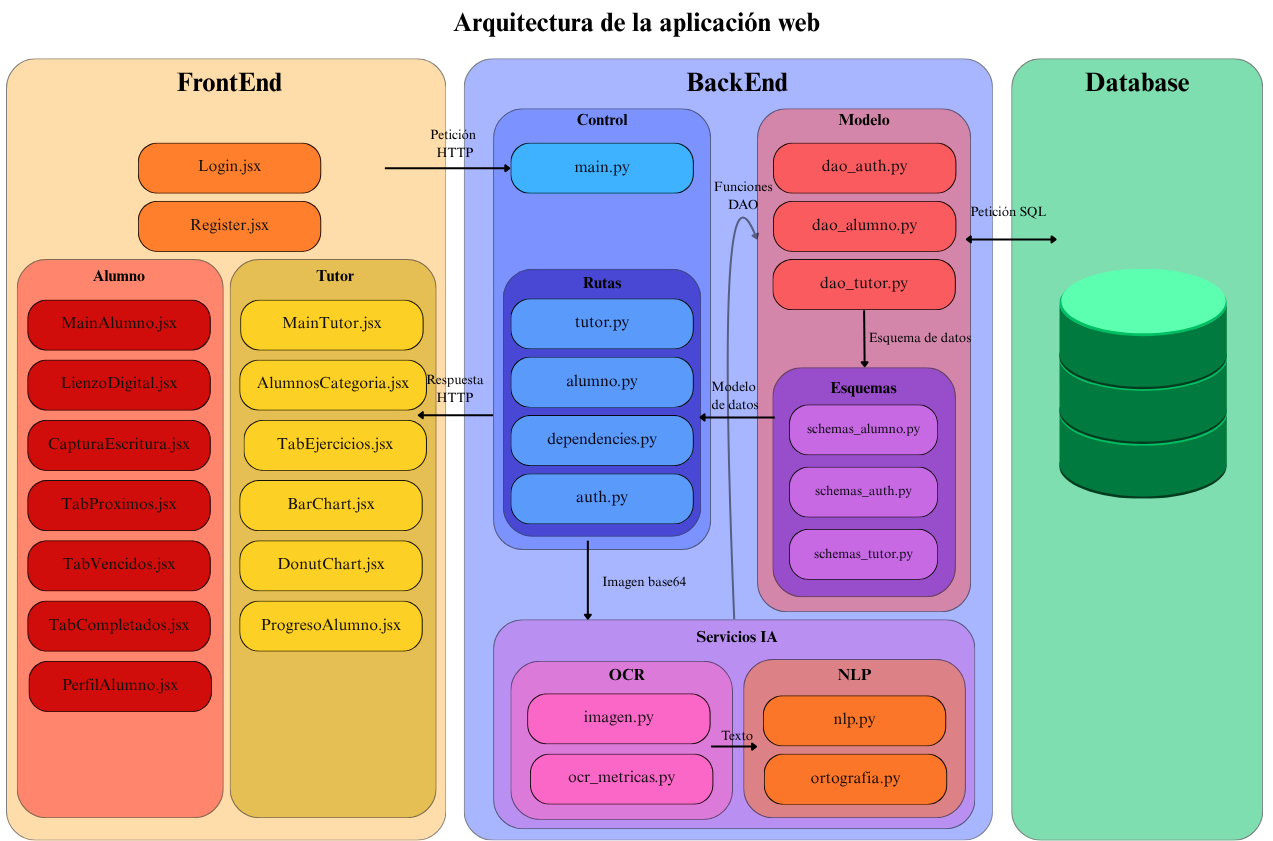
\includegraphics[width=0.95\linewidth]{Imagenes/Arquitectura.png}
        \caption{Diagrama de arquitectura del sistema}
        \label{fig:arquitectura_completa}
    \end{figure}
\end{landscape}